\documentclass[12t,letterpaper]{article}

\newenvironment{proof}{\noindent{\bf Proof:}}{\qed\bigskip}

\newtheorem{theorem}{Theorem}
\newtheorem{corollary}{Corollary}
\newtheorem{lemma}{Lemma} 
\newtheorem{claim}{Claim}
\newtheorem{fact}{Fact}
\newtheorem{definition}{Definition}
\newtheorem{assumption}{Assumption}
\newtheorem{observation}{Observation}
\newtheorem{example}{Example}
\newcommand{\qed}{\rule{7pt}{7pt}}

\newcommand{\assignment}[4]{
\thispagestyle{plain} 
\newpage
\setcounter{page}{1}
\noindent
\begin{center}
\framebox{ \vbox{ \hbox to 6.28in
{\bf EE 122: Communication Networks \hfill #1}
\vspace{4mm}
\hbox to 6.28in
{\hspace{2.5in}\large\mbox{#2}}
\vspace{4mm}
\hbox to 6.28in
{{\it Handed Out: #3 \hfill Due: #4}}
}}
\end{center}
}

\newcommand{\solution}[3]{
\thispagestyle{plain} 
\newpage
\setcounter{page}{1}
\noindent
\begin{center}
\framebox{ \vbox{ \hbox to 6.28in
{\bf EE 122 \hfill #3}
\vspace{4mm}
\hbox to 6.28in
{\hspace{2.5in}\large\mbox{#2}}
\vspace{4mm}
\hbox to 6.28in
{#1 \hfill}
}}
\end{center}
\markright{#1}
}

\newenvironment{algorithm}
{\begin{center}
\begin{tabular}{|l|}
\hline
\begin{minipage}{1in}
\begin{tabbing}
\quad\=\qquad\=\qquad\=\qquad\=\qquad\=\qquad\=\qquad\=\kill}
{\end{tabbing}
\end{minipage} \\
\hline
\end{tabular}
\end{center}}

\def\Comment#1{\textsf{\textsl{$\langle\!\langle$#1\/$\rangle\!\rangle$}}}


\usepackage{amsmath, dsfont, tikz, float}

\usetikzlibrary{arrows,automata,positioning}

\oddsidemargin 0in
\evensidemargin 0in
\textwidth 6.5in
\topmargin -0.5in
\textheight 9.0in

\newenvironment{amatrix}[1]{%
  \left(\begin{array}{@{}*{#1}{c}|c@{}}
}{%
  \end{array}\right)
}

\makeatletter
\renewcommand*\env@matrix[1][*\c@MaxMatrixCols c]{%
  \hskip -\arraycolsep
  \let\@ifnextchar\new@ifnextchar
  \array{#1}}
\makeatother

\newcommand{\norm}[1]{\left\lVert #1 \right\rVert}
\newcommand{\?}{\stackrel{?}{=}}
\newcommand\given[1][]{\:#1\vert\:}


\begin{document}

\solution{Nikhil Unni}{HW1}{Spring 2016}
\pagestyle{myheadings}

\begin{enumerate}
  \item If we order the edges as : $v_1v_2, v_1v_3, v_1v_4, v_1v_5, v_2v_3, v_3v_4, v_4v_5$, and keep the order of vertices, then the incidence matrix becomes:
    $$
      \begin{pmatrix}[ccccccc]
        1 & 1 & 1 & 1 & 0 & 0 & 0\\
        1 & 0 & 0 & 0 & 1 & 0 & 0\\
        0 & 1 & 0 & 0 & 1 & 1 & 0\\
        0 & 0 & 1 & 0 & 0 & 1 & 1\\
        0 & 0 & 0 & 1 & 0 & 0 & 1\\
      \end{pmatrix}
    $$

  \item Running Dijkstra's Algorithm on the graph yields very similar results to just a naïve BFS, except that node 6 is updated. Running Dijkstra's Algorithm, we end up with a table like:
    \begin{center}
      \begin{tabular}{ l | c | r }
        Node & Shortest Distance & Previous Node\\
        \hline
        1 & 3 & 2 \\
        2 & 1 & 3 \\
        3 & 0 &   \\
        4 & 8 & 3 \\
        5 & 7 & 1 \\
        6 & 9 & 5 \\
        7 & 6 & 1 \\
      \end{tabular}
    \end{center}
    Following the paths backwards to node 3, we can construct node 3's routing table:
    \begin{center}
      \begin{tabular}{ l | r}
        Destination & Next\\
        \hline
        1 & 2 \\
        2 & 2 \\
        3 &   \\
        4 & 4 \\
        5 & 2 \\
        6 & 2 \\
        7 & 2 \\
      \end{tabular}
    \end{center}
    
  \item Spanning and Steiner Trees
    \begin{enumerate}
      \item [3.1] A Spanning Tree is a subgraph of a graph that includes every node, but does not have any cycles (i.e. is a valid tree). A Minimum Spanning Tree is the Spanning Tree (since Spanning Trees are not unique) with the least total sum of the edge weights in the tree.
      \item [3.2] The difference between a Steiner Tree and a Spanning Tree is that you may add extra edges and nodes to the original graph when constructing the Steiner Tree (in order to reduce the total cost of the resulting tree).
      \item [3.3] 

        The total cost of the minimum spanning tree (run using Kruskal's Algorithm) is \textbf{42}.
        \begin{figure}[H]
          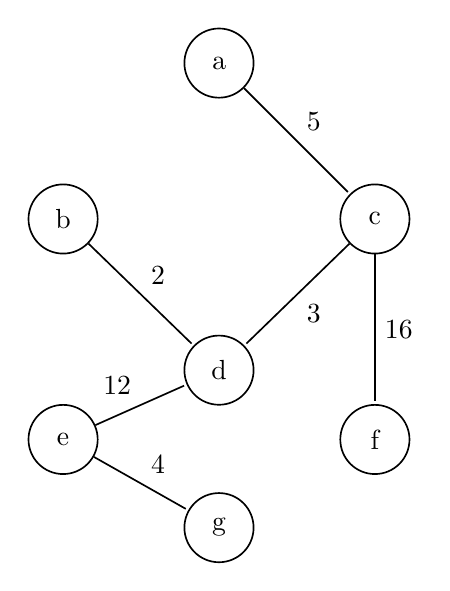
\begin{tikzpicture}[>=stealth',shorten >=1pt,auto,node distance=2.8cm, semithick]
            \tikzstyle{every state}=[fill=none,draw=black,text=black]
            \node[state] (A)                    {a};
            \node[state] (C) [below right of=A] {c};
            \node[state] (B) [below left of=A]  {b};
            \node[state] (F) [below of=C]       {f};
            \node[state] (D) [below=3cm of A]   {d};
            \node[state] (E) [below of=B]       {e};
            \node[state] (G) [below=5cm of A]   {g};

            \path (A) edge              node {5}   (C)
                  (B) edge              node {2}   (D)
                  (C) edge              node {16}  (F)
                      edge              node {3}   (D)
                  (E) edge              node {4}   (G)
                      edge              node {12}  (D);

          \end{tikzpicture}
        \end{figure}
    \end{enumerate}


  \item Using Ford-Fulkerson, we find the maximum flow in the graph is given by the following:
    \begin{figure}[H]
      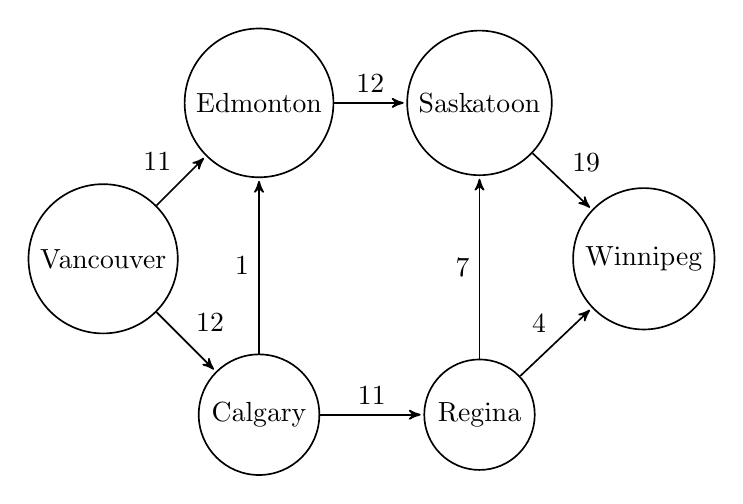
\begin{tikzpicture}[->,>=stealth',shorten >=1pt,auto,node distance=2.8cm, semithick]
        \tikzstyle{every state}=[fill=none,draw=black,text=black]
        \node[state] (A)                    {Vancouver};
        \node[state] (B) [above right of=A] {Edmonton};
        \node[state] (C) [below right of=A] {Calgary};
        \node[state] (D) [right of=B]       {Saskatoon};
        \node[state] (E) [right of=C]       {Regina};
        \node[state] (F) [right=5cm of A]   {Winnipeg};

        \path (A) edge              node {11}  (B)
                  edge              node {12}  (C)
              (B) edge              node {12}  (D)
              (C) edge              node {1}   (B)
                  edge              node {11}  (E)
              (D) edge              node {19}  (F)
              (E) edge              node {7}   (D)
                  edge              node {4}   (F);
                  

      \end{tikzpicture}
    \end{figure}
    So we see that the maximum flow in the graph is \textbf{23}.
  \item 
    \begin{itemize}
      \item [5.1]
        The unreliability of the series is given by:
        $$Q_S = 1 - R_{S1}R_{S2}$$
        The reliability of the parallel components is given by:
        $$R_P = R_{P1} + R_{P2} - R_{P1}R_{P2}$$
        Running these two in series, we get:
        $$Q_{\text{top}} = 1 - (R_{S1}R_{S2})(R_{P1} + R_{P2} - R_{P1}R_{P2})$$
        Finally, putting this together with the bottom, we get:
        $$Q_{\text{system}} = (1 - R_{\text{bottom}})(1 - (R_{S1}R_{S2})(R_{P1} + R_{P2} - R_{P1}R_{P2}))$$

      \item [5.2]
        With m=n=2 and a component reliability of $0.8$, we just plug in the numbers to get:
        $$Q_{\text{system}} = 0.06912$$
        Which means about a $7\%$ error.\\\\

      \item [5.3]
        When n becomes very large, $Q_S$ approaches 1, which means $Q_{\text{top}}$ approaches 1, which means failure of the system is dominated by $Q_{\text{bottom}}$ at the bottom, and will get closer and closer to $Q_{\text{bottom}}$. Similarly, when m becomes very large, $R_P$ approaches 0, and, again, $Q_{\text{top}}$ approaches 1, and failure of the system is dominated by $Q_{\text{bottom}}$.
    \end{itemize}
\end{enumerate}

\end{document}
